\section{Experiments}
\begin{table*}[t]
\caption{VQA accuracy scores on the Encyclopedic-VQA test set and the InfoSeek validation set. The marker $\dagger$ represents our reproductions, while \colorbox{lightgray}{gray color} indicates models tested with non-comparable knowledge bases.}
  \vspace{-0.25cm}
  \centering
  \setlength{\tabcolsep}{.46em}
  \resizebox{\linewidth}{!}{
  \begin{tabular}{lc cc c cc c ccc}
   \toprule
    & & & & & \multicolumn{2}{c}{\textbf{E-VQA}} & & \multicolumn{3}{c}{\textbf{InfoSeek}} \\
    \cmidrule{6-7} \cmidrule{9-11}
     \textbf{Model} & \textbf{Generator} & & \textbf{Retriever} & & Single-Hop & All & & Unseen-Q & Unseen-E & All \\
    \midrule
    BLIP-2~\cite{li2023blip} & - & & - & & 12.6 & 12.4 & & 12.7 & 12.3 & 12.5 \\
    LLaVA-v1.5-7B~\cite{liu2023improved} & - & & - & & 16.3 & 16.9 & & 9.6 & 9.4 & 9.5 \\
    LLaVA-MORE-8B~\cite{cocchi2025llava} & - & & - & & 16.0 & 16.9 & & 8.3 & 8.9 & 7.8 \\
    Qwen2.5-VL-3B~\cite{bai2025qwen2} & - & & - & & 21.9 & 21.9 & & 18.9 & 17.7 & 18.3 \\
    Qwen2.5-VL-7B~\cite{bai2025qwen2} & - & & - & & 23.6 & 23.2 & & 22.8 & 24.1 & 23.7 \\
    \midrule
    \rowcolor{lightgray} 
    DPR$_\text{V+T}$~\cite{lerner2024cross} & Multi-passage BERT & & CLIP ViT-B/32 & & 29.1 & - & & - & - & 12.4 \\
    \rowcolor{lightgray} 
    RORA-VLM~\cite{qi2024rora} & LLaVA-v1.5-7B & & CLIP ViT-L/14 & & - & 20.3 & & 25.1 & 27.3 & - \\
    \rowcolor{lightgray} 
    EchoSight~\cite{yan2024echosight} & Mistral-7B/LLaMA-3-8B & & EVA-CLIP-8B & & 41.8 & - & & - & - & 31.3 \\
    \rowcolor{lightgray}
    CoMEM~\cite{wu2025towards} & Qwen2.5-VL-7B & & Custom VLM & & - & - & & 32.8 & 28.5 & - \\
    Wiki-LLaVA~\cite{caffagni2024wiki} & LLaVA-v1.5-7B & & CLIP ViT-L/14+Contriever & & 17.7 & 20.3 & & 30.1 & 27.8 & 28.9 \\
    EchoSight~\cite{yan2024echosight} & LLaMA-3.1-8B & & EVA-CLIP-8B & & 36.3 & 34.2 & & 30.0 & 30.7 & 30.4 \\
    ReflectiVA~\cite{cocchi2025augmenting} & LLaVA-MORE-8B & & EVA-CLIP-8B & & 35.5 & 35.5 & & 40.4 & 39.8 & 40.1 \\
    mR$^\text{2}$AG~\cite{zhang2024mr} & LLaVA-v1.5-7B & & CLIP ViT-L/14 & & - & - & & 40.6 & 39.8 & 40.2 \\
    VLM-PRF~\cite{hong2025knowledge} & LLaVA-MORE-8B & & EVA-CLIP-8B & & 36.3 & 35.5 & & 41.3 & 40.6 & 40.8 \\
    mKG-RAG~\cite{yuan2025mkg} & LLaVA-MORE-8B & & Custom VLM & & 38.4 & 36.3 & & 41.4 & 39.6 & 40.5 \\
    \midrule
    ReflectiVA~\cite{cocchi2025augmenting}\textsuperscript{\small$\dagger$} & Qwen2.5-VL-3B & & EVA-CLIP-8B & & 33.7 & 35.2 & & 39.6 & 38.1 & 38.9 \\
    VLM-PRF~\cite{hong2025knowledge} & Qwen2.5-VL-3B & & EVA-CLIP-8B & & 31.1 & 32.4 & & 39.7 & 38.8 & 39.0 \\
    \rowcolor{OurColor}
     &  & &  & & \textbf{41.3} & \textbf{42.9} & & \textbf{43.7} & \textbf{42.9} & \textbf{43.3} \\
    \rowcolor{OurColor}
   \multirow{-2}{*}{\textbf{\ours (Ours)}} & \multirow{-2}{*}{Qwen2.5-VL-3B} & & \multirow{-2}{*}{EVA-CLIP-8B} & & \inc{7.6} & \inc{7.7} & & \inc{4.0} & \inc{4.1} & \inc{4.3} \\
    \midrule
    ReflectiVA~\cite{cocchi2025augmenting}\textsuperscript{\small$\dagger$}  & Qwen2.5-VL-7B & & EVA-CLIP-8B & & 36.8 & 36.8 & & 43.5 & 44.3 & 43.9 \\
    
    VLM-PRF~\cite{hong2025knowledge} & Qwen2.5-VL-7B & & EVA-CLIP-8B & & 37.1 & 36.0 & & 43.3 & 42.7 & 42.8 \\
    VLM-PRF~\cite{hong2025knowledge} & InternVL3-8B & & EVA-CLIP-8B & & 40.1 & 39.2 & & 43.5 & 42.1 & 42.5 \\
    \rowcolor{OurColor}
     &  & &  & & \textbf{44.9} & \textbf{47.0} & & \textbf{48.3} & \textbf{46.2} & \textbf{47.2} \\ 
    \rowcolor{OurColor}
   \multirow{-2}{*}{\textbf{\ours (Ours)}} & \multirow{-2}{*}{Qwen2.5-VL-7B} & & \multirow{-2}{*}{EVA-CLIP-8B} & & \inc{4.8} & \inc{7.8} & & \inc{4.8} & \inc{1.9} & \inc{3.3} \\
  \bottomrule
  \end{tabular}
  }
\label{tab:results}
\vspace{-0.45cm}
\end{table*}



\subsection{Datasets and Evaluation Metrics}

\tinytit{Encyclopedic-VQA}
The Encyclopedic-VQA~\cite{mensink2023encyclopedic}
dataset contains 221k question-answer pairs, each linked to up to five images and covering 16.7k fine-grained entities.  
The questions are categorized into \textit{single-hop} and \textit{two-hop} types: single-hop questions can be answered using information from a single Wikipedia page, whereas two-hop questions require sequential retrieval across multiple pages. The dataset is divided into training, validation, and test splits comprising 1M, 13.6k, and 5.8k samples. All experiments are conducted on the test split, which includes 4.8k single-hop questions. The dataset contains an external knowledge base derived from Wikipedia, consisting of approximately 2M pages. Each comprises the article title, its textual sections, and associated images. In our experiments, we employ the original 2M-page knowledge base provided with the dataset.

\tit{InfoSeek} The InfoSeek dataset~\cite{chen2023can} consists of approximately 1.3M image-question-answer triplets corresponding to around 11k distinct Wikipedia pages. It is partitioned into training, validation, and test splits, containing roughly 934k, 73k, and 348k samples. Both validation and test sets include questions about unseen entities.
InfoSeek provides an external knowledge base of around 6M Wikipedia entities. Following previous works~\cite{caffagni2024wiki,cocchi2025augmenting,yan2024echosight}, experiments are conducted using a knowledge base of 100k pages.

\tit{Evaluation Metrics} 
We follow the original evaluation protocols provided with each dataset. For E-VQA, generated answers are evaluated using the BERT-based matching score (BEM)~\cite{bulian2022tomayto}, which measures semantic similarity of predicted and ground-truth answers. For InfoSeek, evaluation depends on the question type: we employ standard VQA accuracy~\cite{goyal2017making} as well as relaxed accuracy~\cite{methani2020plotqa}.


\subsection{Implementation Details}
\label{subsec:details}

\tinytit{Retrieval Details}
To retrieve potentially informative documents for a query image, we employ EVA-CLIP-8B~\cite{sun2024eva}. 
In the coarse-grained stage, the entire query image is encoded through EVA-CLIP to perform large-scale retrieval over the knowledge base.
For InfoSeek, we use an image-to-text retrieval setup that computes similarity between the query image and document metadata (\ie, the title of the page and the summary). For Encyclopedic-VQA, we adopt image-to-image retrieval, comparing the query image with the images inside Wikipedia pages.
In the fine-grained stage, we extract the main visual subject mentioned in the question using the spaCy library\footnote{\url{https://github.com/explosion/spaCy}} and localize it in the image via GroundingDINO~\cite{liu2023grounding}, whose bounding box is re-encoded through EVA-CLIP. Retrieval is done using the FAISS library~\cite{johnson2019billion}, with the top-$k$ results with $k=20$ retained at each stage.

\tit{Critic Model and Dataset}
Independently from the generator scale, our critic model builds upon Qwen2.5-VL-3B, fine-tuned on a curated subset of the ReflectiVA dataset~\cite{cocchi2025augmenting}\footnote{Further details on the training subset are given in the supplementary.}.
The model is trained for 1 epoch with a learning rate of $2 \times 10^{-6}$ and a global batch size of $32$.

\tit{Generator Training}
We build two versions of our generator, both based on Qwen2.5-VL~\cite{bai2025qwen2}, using the 3B and 7B model variants, and optimize them using the SFT plus RL training scheme. In the SFT phase, we use the same ReflectiVA~\cite{cocchi2025augmenting} subset employed to train the critic model, collecting reasoning traces from Qwen2.5-VL-7B. We set $\alpha=0.8$ to give more importance to final-answer tokens. The generator is trained for one epoch with SFT loss using AdamW~\cite{loshchilovdecoupled},
a learning rate of $2\times10^{-6}$ and an effective batch size of 128.
For RL post-training, we use the full Encyclopedic-VQA and InfoSeek sets from ReflectiVA, excluding samples from LLaVA-Instruct~\cite{liu2023improved}. Each batch includes 128 prompts with 8 completions per prompt. 
Training is conducted with Adam~\cite{kingma2015adam}, a learning rate $1\times10^{-6}$. Rewards weigh accuracy $\gamma=1.0$ over format $\delta=0.2$.
In all our experiments, we update the MLP adapter and LLM weights while keeping the vision encoder frozen. 

\subsection{Comparison with the State of the Art}
\begin{table}[t]
\caption{VQA accuracy scores on Encyclopedic-VQA and InfoSeek with OMGM as retrieval modality.}
\label{tab:results3}
  \vspace{-0.25cm}
  \centering
  \setlength{\tabcolsep}{.25em}
  \resizebox{\linewidth}{!}{
  \begin{tabular}{lc c cc c ccc}
   \toprule
    & & & \multicolumn{1}{c}{\textbf{E-VQA}}& & \multicolumn{3}{c}{\textbf{InfoSeek}} \\
    \cmidrule{4-4} \cmidrule{6-8}
     \textbf{Model} & \textbf{Generator} & & Single-Hop & & Un-Q & Un-E & All \\
    \midrule
    ReflectiVA~\cite{cocchi2025augmenting} & LLaVA-MORE-8B & & 41.8 & & 33.8 & 34.5 & 34.1 \\
    OMGM~\cite{yang2025omgm} & LLaVA-v1.5-7B & & 50.2 & & 43.5 & 43.5 & 43.5 \\
   \midrule
    ReflectiVA~\cite{cocchi2025augmenting} & Qwen2.5-VL-3B & & 44.6 & & 40.5 & 41.6 & 41.1 \\
      \rowcolor{OurColor}
    \textbf{\ours (Ours)} & Qwen2.5-VL-3B & & \textbf{49.1} & & \textbf{47.2} & \textbf{45.3} & \textbf{46.2} \\
    \midrule
    ReflectiVA~\cite{cocchi2025augmenting} & Qwen2.5-VL-7B & & 44.0 & & 43.3 & 44.0 & 43.6 \\
  
    \rowcolor{OurColor}
    \textbf{\ours (Ours)} & Qwen2.5-VL-7B & & \textbf{52.5} & & \textbf{50.3} & \textbf{48.2} & \textbf{49.2} \\
  \bottomrule
  \end{tabular}
  }
\vspace{-0.25cm}
\end{table}


\tinytit{Main Results} 
We present a comprehensive comparison of \ours on the E-VQA test set and the InfoSeek validation set against both zero-shot MLLMs and retrieval-augmented baselines. Specifically, we evaluate BLIP-2~\cite{li2023blip}, LLaVA-v1.5~\cite{liu2023improved}, LLaVA-MORE~\cite{cocchi2025llava}, and Qwen2.5-VL~\cite{bai2025qwen2} in a zero-shot setting, where the models receive only the query image and question as input. We further include retrieval-augmented approaches such as DPR~\cite{lerner2024cross}, RORA-VLM~\cite{qi2024rora}, EchoSight~\cite{yan2024echosight}, COMEM~\cite{wu2025towards}, WikiLLaVA~\cite{caffagni2024wiki}, mR$^\text{2}$AG~\cite{zhang2024mr}, mKG-RAG~\cite{yuan2025mkg}, ReflectiVA~\cite{cocchi2025augmenting}, and VLM-PRF~\cite{hong2025knowledge}. For fairness, we reproduce ReflectiVA using Qwen2.5-VL backbones at both 3B and 7B scales.

As shown in Table~\ref{tab:results}, zero-shot MLLMs, which rely solely on internal knowledge, are unable to accurately answer questions in knowledge-intensive benchmarks, underscoring the need for external retrieval. With the introduction of a retrieval pipeline, performance improves substantially. For example, on InfoSeek, the overall accuracy rises from around $20\%$ for the zero-shot Qwen2.5-VL-7B model to roughly $40\%$ with retrieval-augmented methods such as mKG-RAG. \ours further advances these results, achieving state-of-the-art performance on both E-VQA and InfoSeek across model scales. Specifically, on E-VQA \ours yields a $+7.7$ point gain over ReflectiVA when using Qwen2.5-VL-3B and a $+7.8$ point improvement over VLM-PRF when leveraging the stronger InternVL3-8B backbone.
Similar gains are observed on InfoSeek, with overall improvements of $+4.3$ and $+3.3$ points for Qwen2.5-VL-3B and 7B, respectively. These consistent improvements across both datasets demonstrate the effectiveness and robustness of our approach.





\begin{table}[t]
\caption{VQA accuracy scores on Encyclopedic-VQA and InfoSeek with oracle Wikipedia pages. }
  \label{tab:results_oracle}
    \vspace{-0.25cm}
  \centering
  \setlength{\tabcolsep}{.18em}
  \resizebox{\linewidth}{!}{
  \begin{tabular}{lcc c c ccc}
   \toprule
    & & & \multicolumn{1}{c}{\textbf{E-VQA}} & & \multicolumn{3}{c}{\textbf{InfoSeek}} \\
    \cmidrule{4-4} \cmidrule{6-8}
    \textbf{Model} & \textbf{Generator} & & Single-Hop & & Un-Q & Un-E & All \\
    \midrule
    Qwen2.5-VL-3B~\cite{bai2025qwen2} & Qwen2.5-3B & & 72.1 & & 47.0 & 43.0 & 44.9 \\
    Qwen2.5-VL-7B~\cite{bai2025qwen2} & Qwen2.5-7B & & 78.3 & & 41.6 & 41.3 & 41.4 \\
    \midrule
    ReflectiVA~\cite{cocchi2025augmenting} & Qwen2.5-VL-3B & & 72.9 & & 53.4 & \textbf{53.9} & 53.7 \\
    \rowcolor{OurColor}
    \textbf{\ours (Ours)} & Qwen2.5-VL-3B & & \textbf{79.0} & & \textbf{55.1} & 53.3 & \textbf{54.2} \\
    \midrule
    Wiki-LLaVA~\cite{caffagni2024wiki} & LLaVA-v1.5-7B & & 38.5 & & 52.7 & 50.3 & 51.5 \\
    
    ReflectiVA~\cite{cocchi2025augmenting} & LLaVA-MORE-8B & & 75.2 & & 57.8 & 57.4 & 57.6 \\
    ReflectiVA~\cite{cocchi2025augmenting} & Qwen2.5-VL-7B & & 71.3 & & 56.0 & 56.0 & 56.0 \\
    \rowcolor{OurColor}
    \textbf{\ours (Ours)} & Qwen2.5-VL-7B & & \textbf{81.5} & & \textbf{60.7} & \textbf{58.9} & \textbf{59.7} \\
  \bottomrule
  \end{tabular}
  }
\vspace{-0.35cm}
\end{table}


\begin{figure}
    \centering
    \includegraphics[width=0.99\linewidth]{images/inverted_combined_plot_legend_18.pdf}
    \vspace{-0.3cm}
    \caption{Comparison of performance on E-VQA with and without evidence, including oracle upper bounds (left). Analysis on average number of passages retained at different top‑$k$ values (right).}
    \label{fig:graphs}
    \vspace{-0.3cm}
\end{figure}

\begin{table*}[t]
\caption{Ablation study results on Encyclopedic-VQA and InfoSeek to validate the effectiveness of our model component.}
  \vspace{-0.2cm}
  \centering
  \setlength{\tabcolsep}{.25em}
  \resizebox{\linewidth}{!}{
  \begin{tabular}{lc cc ccc c cccc c c c ccc}
   \toprule
     & && \multicolumn{3}{c}{\textbf{Retrieval Pipeline}} & & \multicolumn{3}{c}{\textbf{Generation Pipeline}} & & \multicolumn{1}{c}{\textbf{E-VQA}} & & \multicolumn{3}{c}{\textbf{InfoSeek}} \\
     \cmidrule{4-6} \cmidrule{8-10} \cmidrule{12-12} \cmidrule{14-16}
      & \textbf{Generator} && Coarse-grained & Fine-grained & Critic & & SFT & Reasoning Traces & RL & & Single-Hop & & Unseen-Q & Unseen-E & All \\
     \midrule 
     &  && - & - & - & & - & - & - & & 21.9 & & 18.9 & 17.7 & 18.3 \\
    & && \cmark & - & - & & - & - & - & & 19.2 & & 10.2 & 10.0 & 10.1 \\
    & && \cmark & - & \cmark & & - & - & - & & 38.0 & & 27.9 & 26.1 & 27.0 \\
    & && \cmark & \cmark & \cmark & & - & - & - & & 40.2 & & 28.1 & 26.1 & 27.1 \\
    \midrule   
    & && \cmark & \cmark & \cmark & & \cmark & - & - & & 39.3 & & 37.9 & 37.1 & 37.5 \\
    & && \cmark & \cmark & \cmark & & \cmark & \cmark & - & & 38.1 & & 41.9 & 40.6 & 41.3 \\
    & && \cmark & \cmark & \cmark & & \cmark & - & \cmark & & 39.5 & & 39.8 & 39.4 & 39.6 \\
    \rowcolor{OurColor}
    \textbf{\ours (Ours)} & Qwen2.5-VL-3B && \cmark & \cmark & \cmark & & \cmark & \cmark & \cmark & & \textbf{41.3} & & \textbf{43.7} & \textbf{42.9} & \textbf{43.3} \\
    \midrule
    \midrule
    & && \cmark & \cmark & \cmark & & - & - & - & & 41.7 & & 29.3 & 27.8 & 28.5 \\
    & && \cmark & \cmark & \cmark & & \cmark & \cmark & - & & 42.0 & & 42.0 & 40.7 & 41.4 \\
    \rowcolor{OurColor}
     \textbf{\ours (Ours)}  & Qwen2.5-VL-7B && \cmark & \cmark & \cmark & & \cmark & \cmark & \cmark & & \textbf{44.9} & & \textbf{48.3} & \textbf{46.2} & \textbf{47.2} \\
  \bottomrule
  \end{tabular}
  }
\label{tab:ablation}
\vspace{-0.2cm}
\end{table*}

\begin{figure*}[t]
\begin{minipage}{0.325\linewidth}
\scriptsize{\textbf{Q}: What is the closest upper taxonomy of this bird?\vspace{0.05cm}}\\
\begin{minipage}{0.443\linewidth}
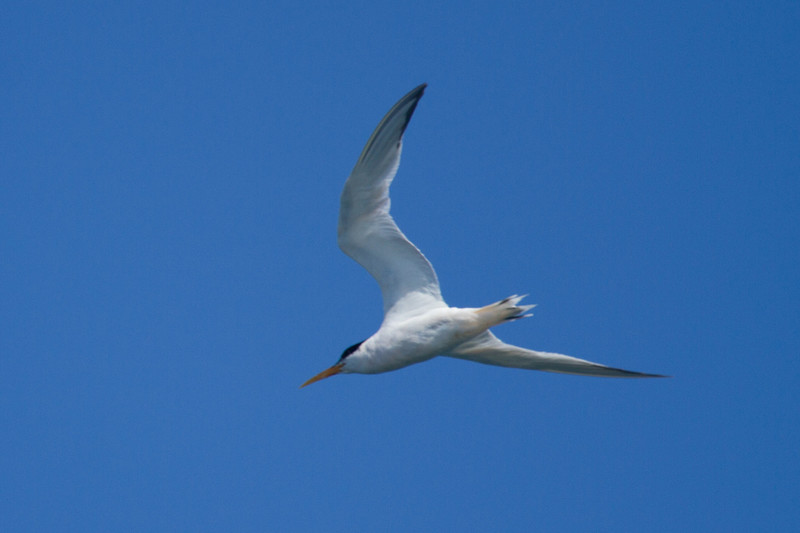
\includegraphics[width=1.\linewidth,height=0.88\linewidth]{images/qualitatives/gabbiano.png}
\end{minipage}
\hfill
\begin{minipage}{0.53\linewidth}
\scriptsize{
\textbf{Qwen2.5-VL-7B (ZS)~\cite{bai2025qwen2}}:\\
The closest taxonomy of this bird is the family Laridae. \textcolor{red}{\xmark} \\
\textbf{ReflectiVA~\cite{cocchi2025augmenting}}:\\
Sterna \textcolor{red}{\xmark} \\
\textbf{\ours (Ours):}\\
Thalasseus\textcolor[HTML]{00b050}{\cmark}
}
\end{minipage}
\end{minipage}
\hspace{0.02cm}
\begin{minipage}{0.325\linewidth}
\scriptsize{\textbf{Q}:Which road, railway or canal does this bridge carry?\vspace{0.05cm}}\\
\begin{minipage}{0.443\linewidth}
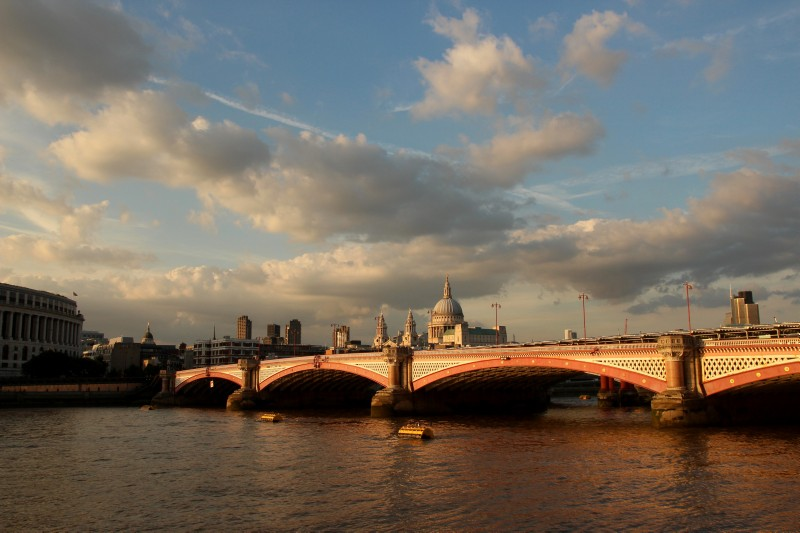
\includegraphics[width=1.\linewidth,height=0.88\linewidth]{images/qualitatives/bridge.png}
\end{minipage}
\hfill
\begin{minipage}{0.53\linewidth}
\scriptsize{
\textbf{Qwen2.5-VL-7B (ZS)~\cite{bai2025qwen2}}:\\
The bridge in the picture is Blackfriars Bridge. \textcolor{red}{\xmark} \\
\textbf{ReflectiVA~\cite{cocchi2025augmenting}}: \\ 
Road \textcolor{red}{\xmark} \\
\textbf{\ours (Ours):}\\
A201 \textcolor[HTML]{00b050}{\cmark}
}
\end{minipage}
\end{minipage}
\hspace{0.02cm}
\begin{minipage}{0.325\linewidth}
\scriptsize{\textbf{Q:} What is the brand of this vehicle? \vspace{0.05cm}}\\
\begin{minipage}{0.443\linewidth}
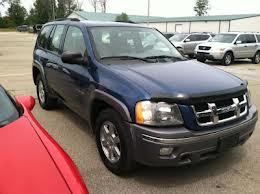
\includegraphics[width=1.\linewidth,height=0.88\linewidth]{images/qualitatives/car.png}
\end{minipage}
\hfill
\begin{minipage}{0.53\linewidth}
\scriptsize{
\textbf{Qwen2.5-VL-7B (ZS)~\cite{bai2025qwen2}}:\\
The vehicle in the picture is a Ford. This can be determined [..] \textcolor{red}{\xmark} \\
\textbf{ReflectiVA~\cite{cocchi2025augmenting}}:\\
Ford \textcolor{red}{\xmark} \\
\textbf{\ours (Ours):}\\
Isuzu \textcolor[HTML]{00b050}{\cmark}
}
\end{minipage}
\end{minipage}
\vspace{-0.25cm}
\caption{Qualitative results on InfoSeek image-question pairs comparing \ours, ReflectiVA~\cite{cocchi2025augmenting}, and the corresponding zero-shot model.}
\label{fig:qualitatives}
\vspace{-0.35cm}
\end{figure*}

\tit{Results with OMGM Retrieval Mode}
We also compare against the OMGM framework~\cite{yang2025omgm}, which adopts a coarse-to-fine, multi-stage retrieval strategy, leveraging an image-to-text summary retriever in the first step.
To ensure a fair comparison, in Table~\ref{tab:results3} we evaluate our method using the same retrieval modality. Notably, our method consistently outperforms OMGM~\cite{yang2025omgm} across both E-VQA and InfoSeek benchmarks.
With the Qwen2.5-VL-3B generator, our approach achieves substantial improvements over ReflectiVA~\cite{cocchi2025augmenting}, yielding gains of $+4.5$ and $+5.1$ points on E-VQA and InfoSeek. 
When scaling to Qwen2.5-VL-7B, performance further increases, reaching $52.5$ on E-VQA and $49.2$ on InfoSeek, surpassing OMGM by $2.3$ and $5.7$ points, respectively. 
These results indicate that, even when using only the initial retrieval step of OMGM, our critic-based filtering, together with \ours reasoning capabilities, leads to consistently higher performance compared to both prior methods and the full multi-stage retrieval of OMGM.

\tit{Results with Oracle Documents} 
We also experiment under an oracle setting (Table~\ref{tab:results_oracle}), where the ground-truth document (\ie, the Wikipedia page corresponding to the query) is provided. 
We compare results from zero-shot models (Qwen2.5-VL~\cite{bai2025qwen2} in both 3B and 7B variants), which take the entire Wikipedia pages as input, and retrieval-based methods (WikiLLaVA~\cite{caffagni2024wiki}, ReflectiVA~\cite{cocchi2025augmenting}, and \ours), which process retrieved passages through an additional model-specific filtering stage. In this configuration, \ours receives all passages from the oracle document, which are then passed to the critic model for filtering before being fed to the generator.

Notably, \ours achieves the best performance across both E-VQA and InfoSeek at all model scales. On the 3B variant, \ours outperforms ReflectiVA by $+6.1$ points on E-VQA, while on Infoseek the 7B version consistently improves over ReflectiVA by $+3.7$ and still surpasses it by $+2.1$ even when ReflectiVA employs a larger generator (LLaVA-MORE-8B).

\tit{Retrieval and Generation Pipeline Analysis} 
The performance of RAG-based approaches strongly depends on the presence of the evidence passage in the retrieved set, and on the number of passages provided to the generator. 

In Fig.~\ref{fig:graphs} (left), we evaluate the ability to produce the correct answer when the evidence passage is either present or absent in the context. \ours consistently outperforms all competitors of comparable scale, demonstrating that our reasoning-enhanced approach is robust even in the absence of direct evidence. Each model is also accompanied by its oracle performance, clearly showing that \ours consistently gets closer to the oracle upper bound than other approaches.

In Fig.~\ref{fig:graphs} (right), we instead report the average number of passages passed to the generation at different $k$ values, comparing the filtering behavior of ReflectiVA~\cite{cocchi2025augmenting} with that of our critic model. \ours reduces noise introduced in the generator context by achieving a reduction of $18.0\%$ and $15.9\%$ in the number of passages compared to ReflectiVA based on LLaVA-MORE-8B and Qwen2.5VL-3B respectively, further emphasizing the advantage of our filtering pipeline.

\tit{Qualitative Results} 
In Fig.~\ref{fig:qualitatives}, we present a qualitative comparison on image-question pairs from InfoSeek. Notably, the zero-shot model tends to produce longer and detailed answers, whereas ReflectiVA and \ours generate responses that follow the dataset-specific format. Overall, the results consistently demonstrate that \ours answers accurate and outperforms competing approaches.


\subsection{Ablation Studies} 
We finally perform an ablation study by progressively enabling key components of the final architecture. Table~\ref{tab:ablation} reports results at each stage with $k$ equal to 20, evaluating the effect of the critic and fine-grained retrieval modules, as well as design choices in the generation pipeline.

We first examine the zero-shot setup under different retrieval configurations, using the 3B-scale model. As shown in the first two rows of Table~\ref{tab:ablation}, directly passing all passages from the top-20 documents into the generator severely degrades performance due to excessive noise. Introducing the critic model (third row) effectively filters irrelevant passages, yielding more than a twofold gain. Adding the fine-grained retriever (fourth row) further improves retrieval recall and yields additional gains on both datasets.

Fixing the retrieval pipeline to its final configuration, we then assess the impact of different generation strategies. As shown in~\cite{guo2025deepseek}, introducing a cold-start phase can help prepare the model for reasoning by exposing it to intermediate traces before full supervision. Results show that applying reinforcement learning after this cold-start phase outperforms standard SFT, indicating that the cold-start phase effectively prepares the model for multi-step reasoning, allowing the RL algorithm to operate on a model already prepared for structured thinking. 
A similar trend is observed with the 7B variant, where both training phases contribute significantly to the final performance, further validating the robustness of the proposed \ours pipeline.
